\section*{Supplementary figures chapter 2}

\begin{figure}[H]
	\centering
	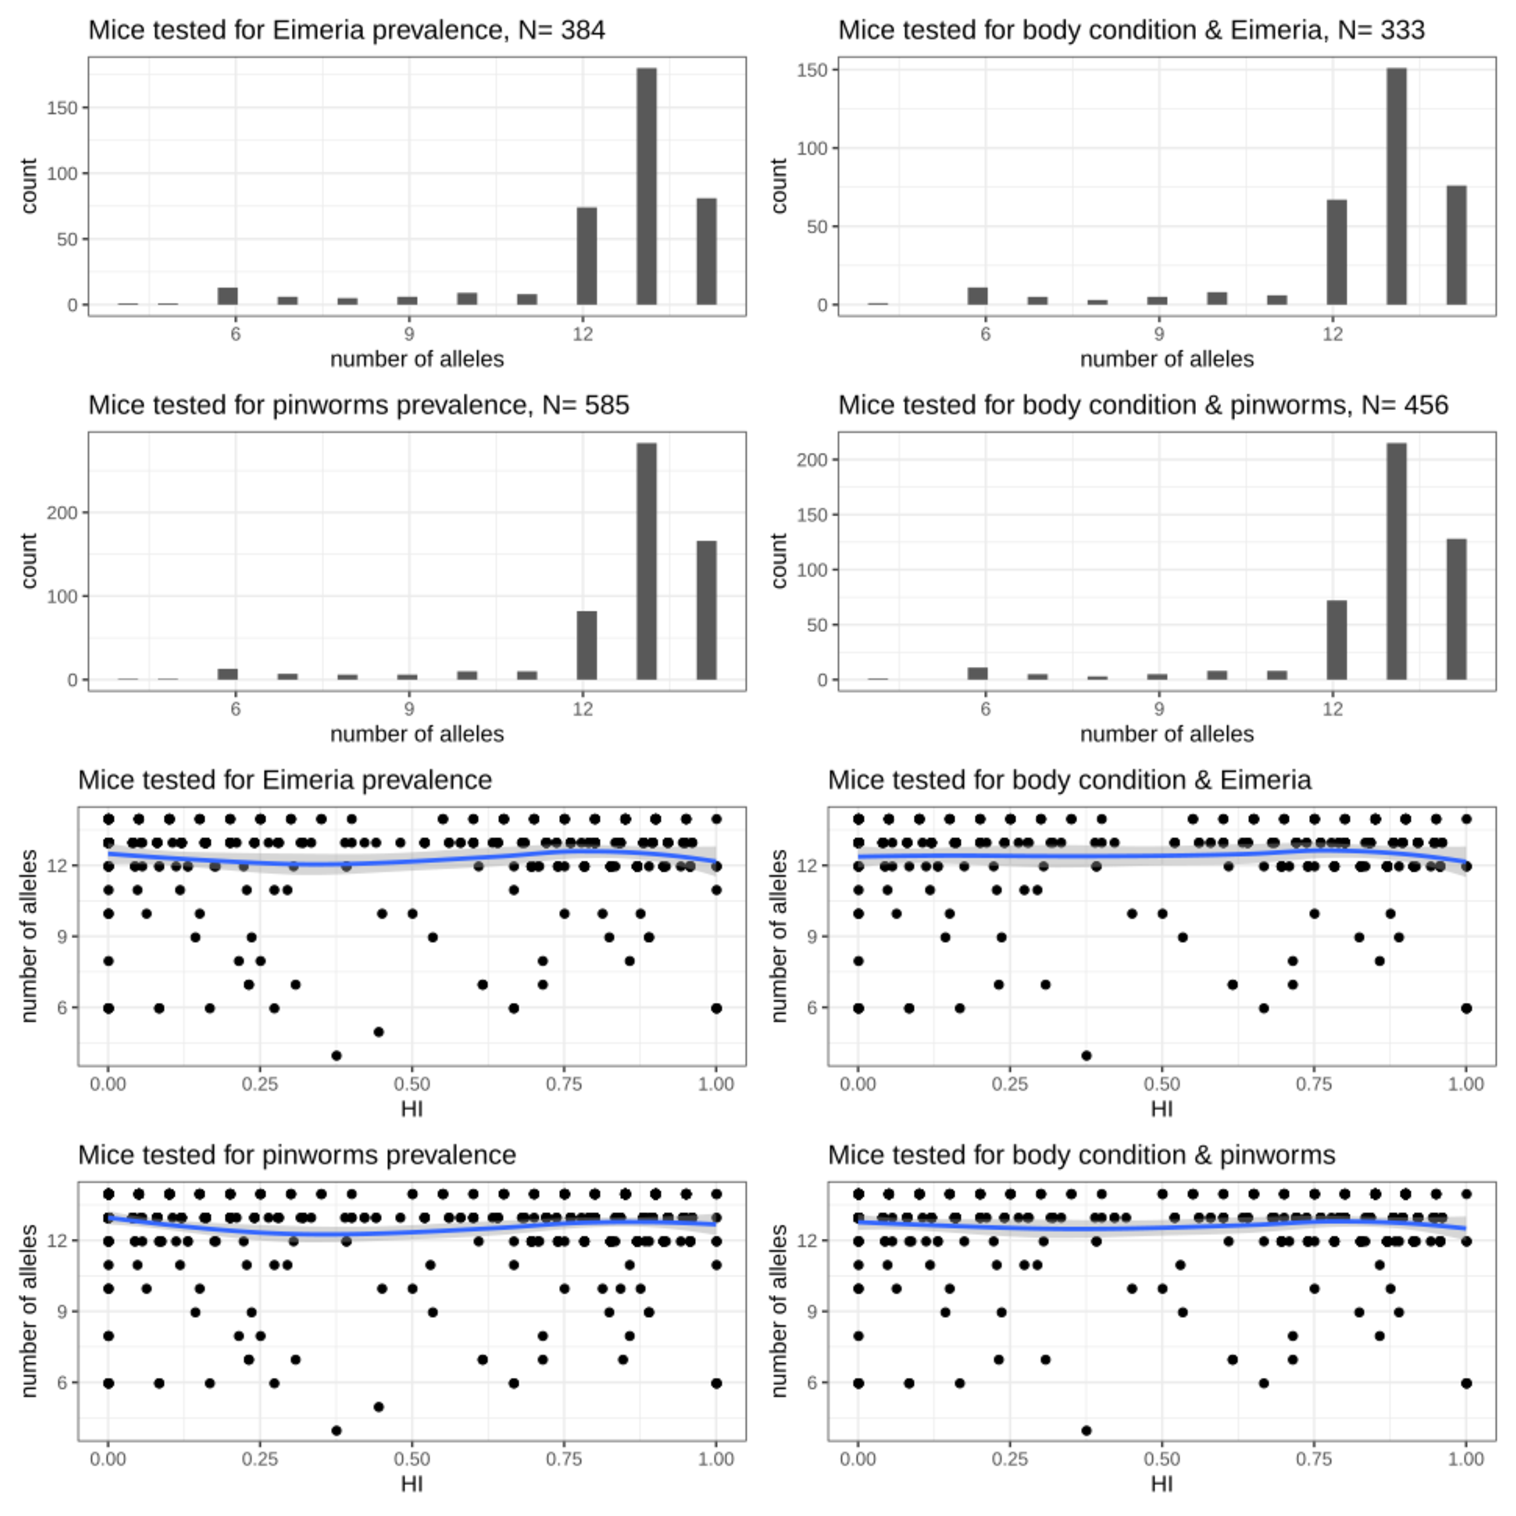
\includegraphics[width=\linewidth,height=\textheight,keepaspectratio]{images/2article1/SupplementaryFigureS1.pdf}
	\captionsetup{labelformat=empty}
	\caption{\textbf{Supplementary Figure S2.1.} Number of markers used for each analysis. Histogram of distribution, and raw data with smooth along hybrid index (HI).}
\end{figure}

\newpage

\begin{figure}[H]
	\centering
	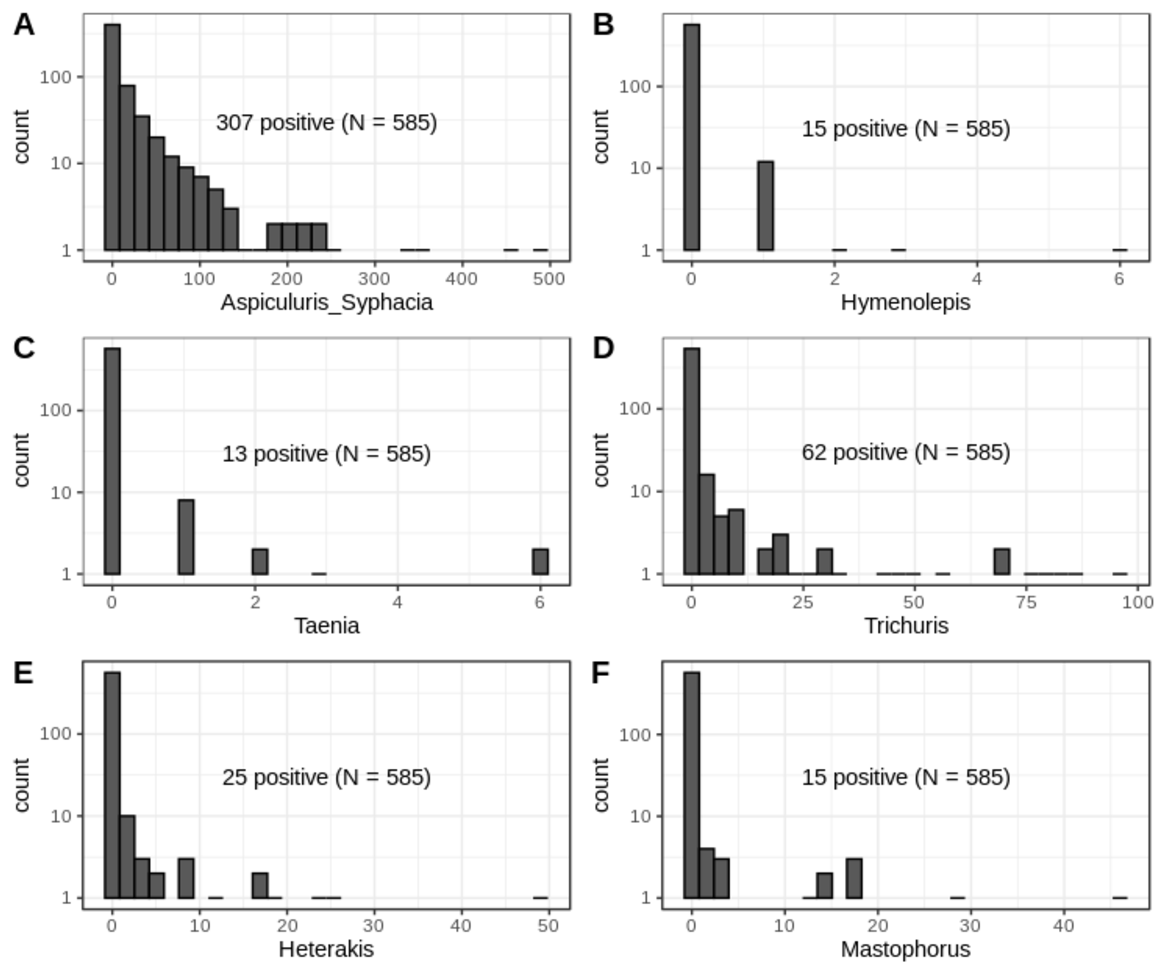
\includegraphics[width=\linewidth,height=\textheight,keepaspectratio]{images/2article1/SupplementaryFigureS2.pdf}
	\captionsetup{labelformat=empty}
	\caption{\textbf{Supplementary Figure S2.2.} Distribution of helminths counts in all mice investigated for worms (N=585).}
\end{figure}

\newpage

\textbf{Supplementary Table S2.3.} Raw data. Table not included in the present thesis; can be downloaded at \url{https://onlinelibrary.wiley.com/doi/full/10.1111/jeb.13578}, in the section Supporting information, jeb13578-sup-0006-TableS3.xlsxMS Excel, 108.8 KB

\newpage

\begin{figure}[H]
	\centering
	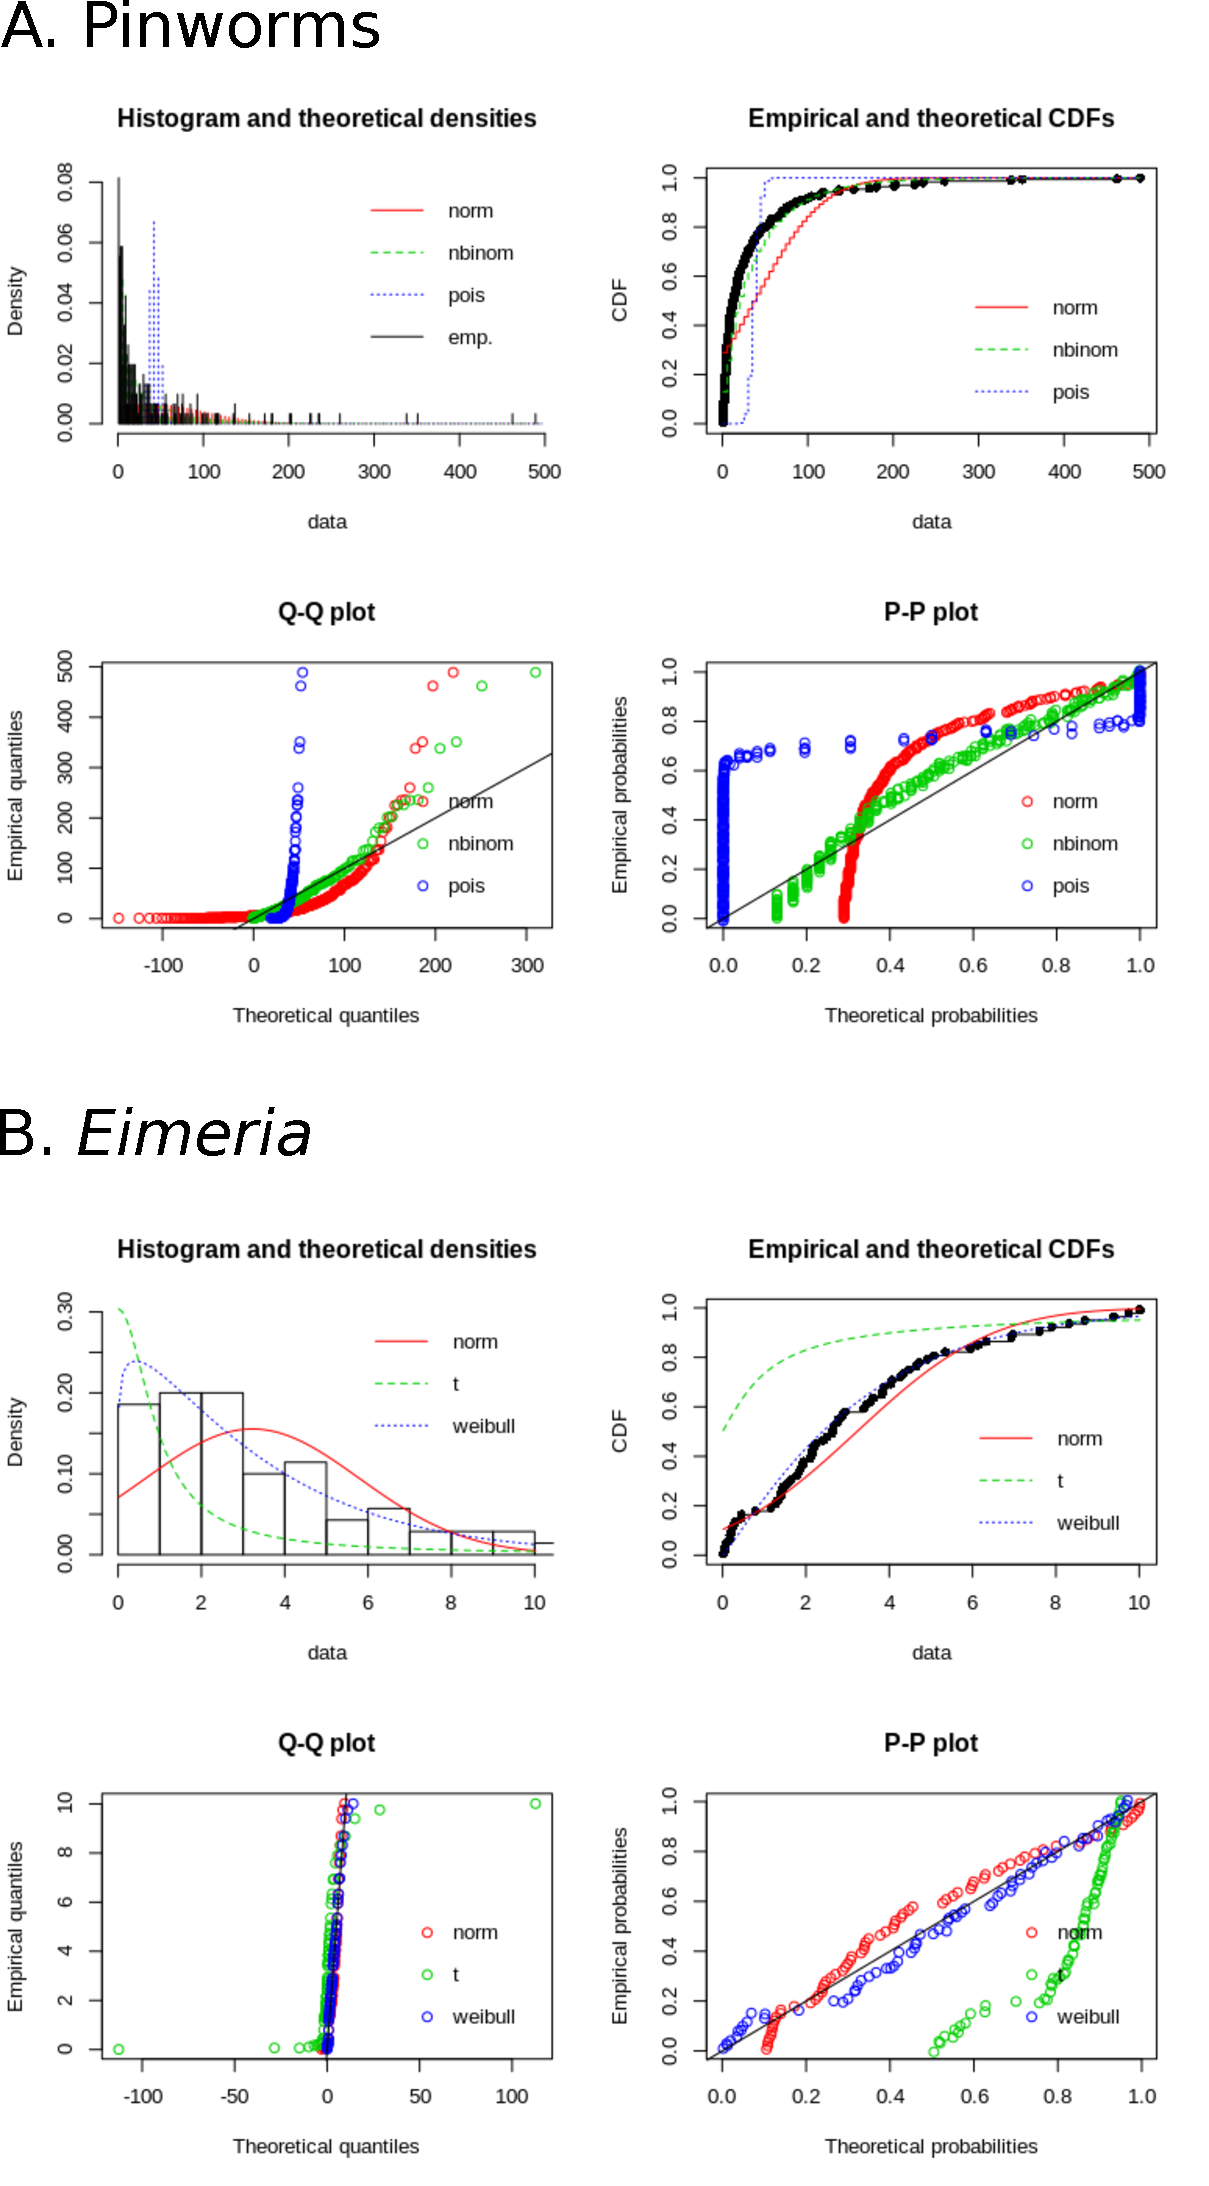
\includegraphics[width=\linewidth,height=\textheight,keepaspectratio]{images/2article1/SupplementaryFigureS4.pdf}
	\captionsetup{labelformat=empty}
	\caption{\textbf{Supplementary Figure S2.4.} Choice of distribution for (positive) parasite loads (intensity).}
\end{figure}

\newpage

\begin{figure}[H]
	\centering
	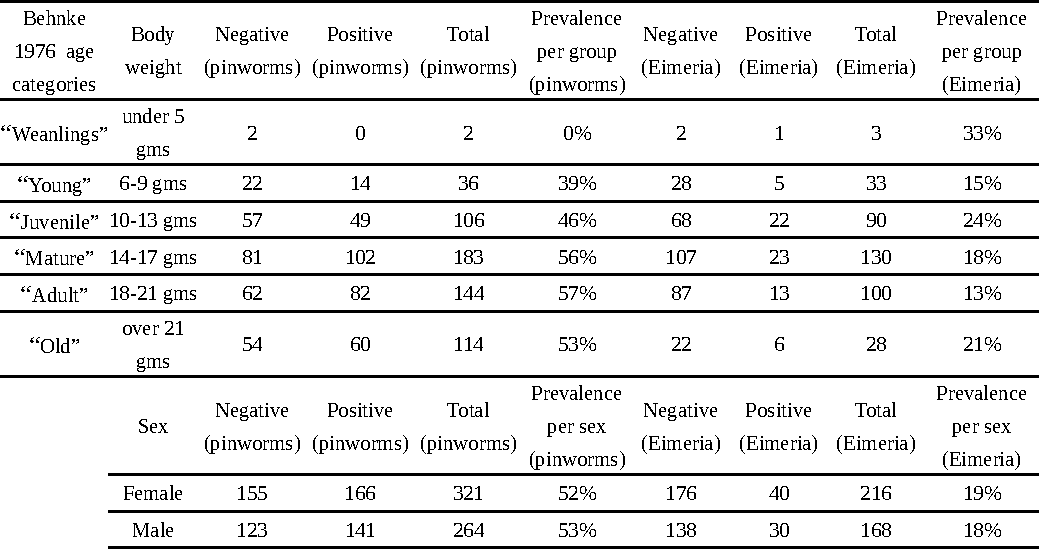
\includegraphics[width=\linewidth,height=\textheight,keepaspectratio]{images/2article1/SupplementaryTableS5.pdf}
	\captionsetup{labelformat=empty}
	\caption{\textbf{Supplementary Table S2.5.} Table of prevalence of pinworms and \textit{Eimeria}~spp. by weight category and sex.}
\end{figure}

\vspace{2cm}

\begin{figure}[H]
	\centering
	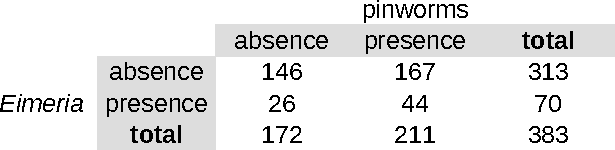
\includegraphics[width=\linewidth,height=\textheight,keepaspectratio]{images/2article1/SupplementaryTableS6.pdf}
	\captionsetup{labelformat=empty}
	\caption{\textbf{Supplementary Table S2.6.}  Contingency table Eimeria/pinworms presence/absence.}
\end{figure}

\newpage

\begin{figure}[H]
	\centering
	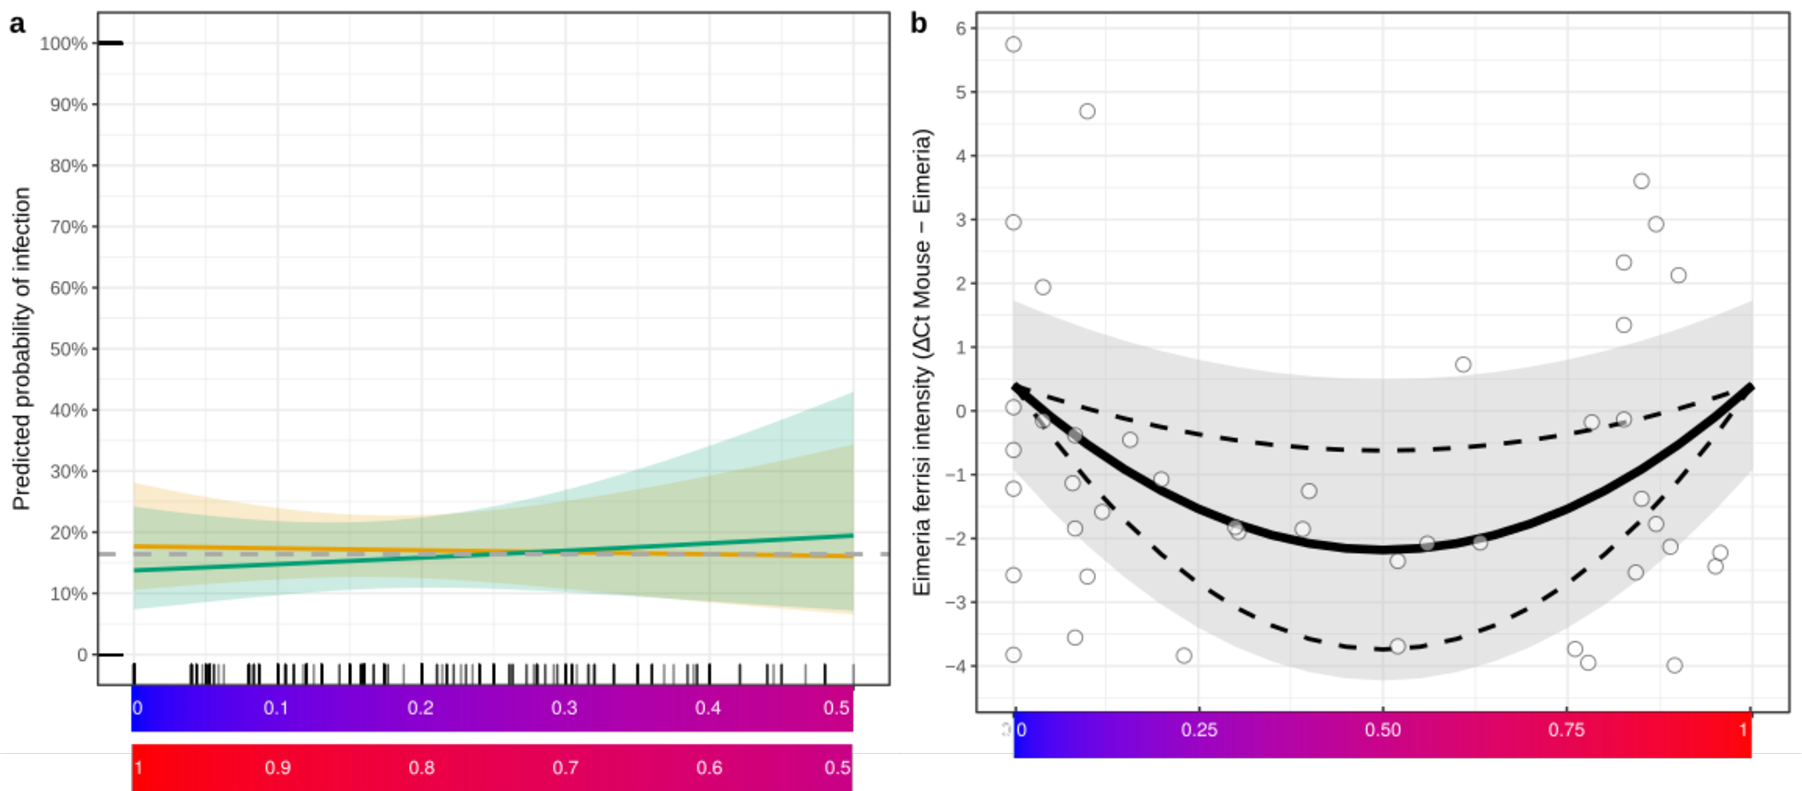
\includegraphics[width=\linewidth,height=\textheight,keepaspectratio]{images/2article1/SupplementaryFigureS7.pdf}
	\captionsetup{labelformat=empty}
	\caption{\textbf{Supplementary Figure S2.7.} Probability of infection is constant and intensity of \textit{Eimeria~ferrisi} infection is reduced in hybrids.}
\end{figure}

\newpage

\begin{figure}[H]
	\centering
	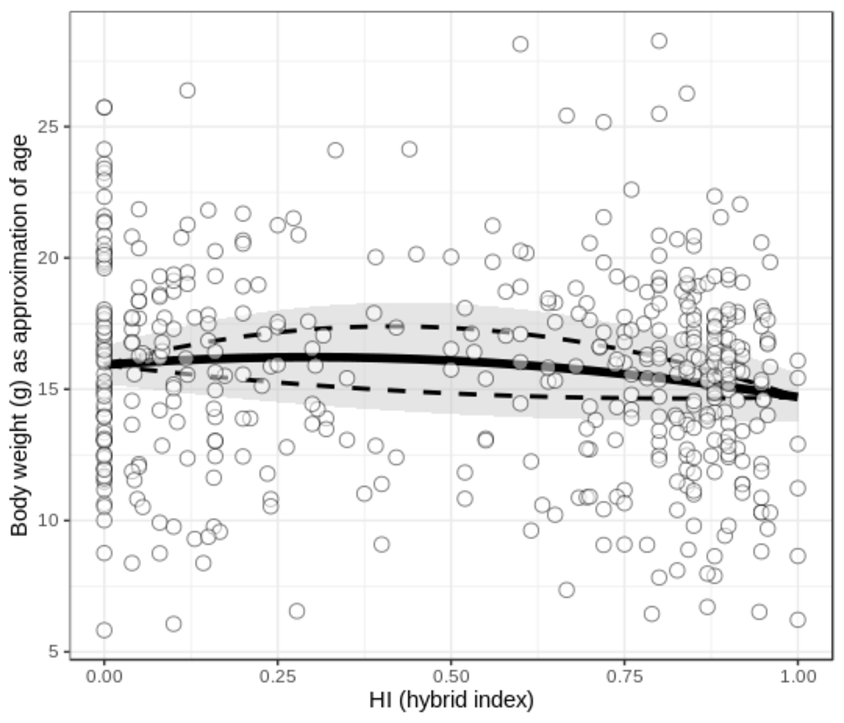
\includegraphics[width=\linewidth,height=\textheight,keepaspectratio]{images/2article1/SupplementaryFigureS8.pdf}
	\captionsetup{labelformat=empty}
	\caption{\textbf{Supplementary Figure S2.8.}  No decrease or increase in mortality in more admixed mice.}
\end{figure}

\newpage

\begin{figure}[H]
	\centering
	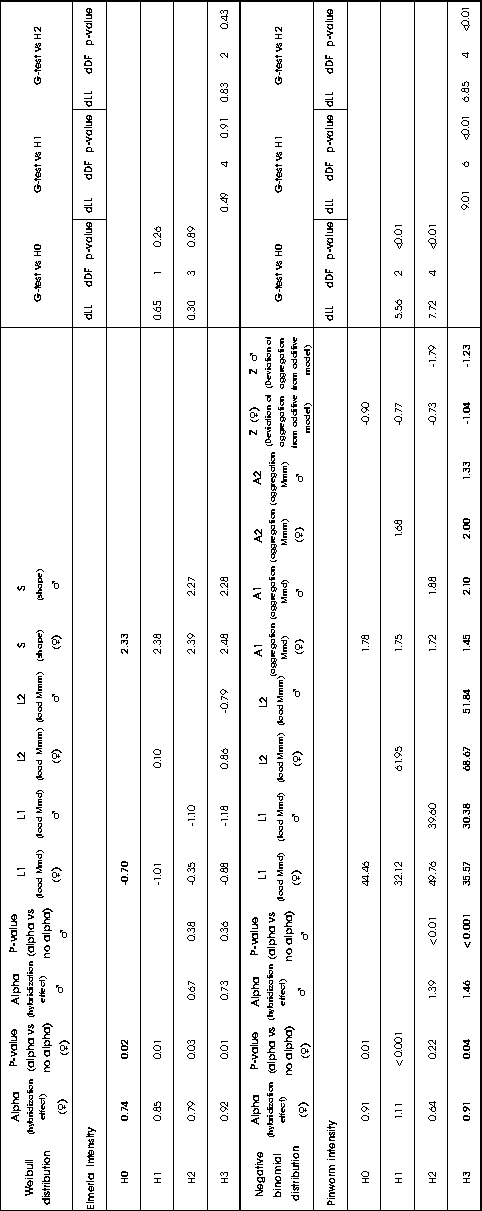
\includegraphics[width=\linewidth,height=\textheight,keepaspectratio]{images/2article1/SupplementaryTableS9.pdf}
	\captionsetup{labelformat=empty}
	\caption{\textbf{Supplementary Table S2.9.} Models full parameters.}
\end{figure}

\newpage

\section*{Supplementary figures chapter 3}

\begin{figure}[H]
	\centering
	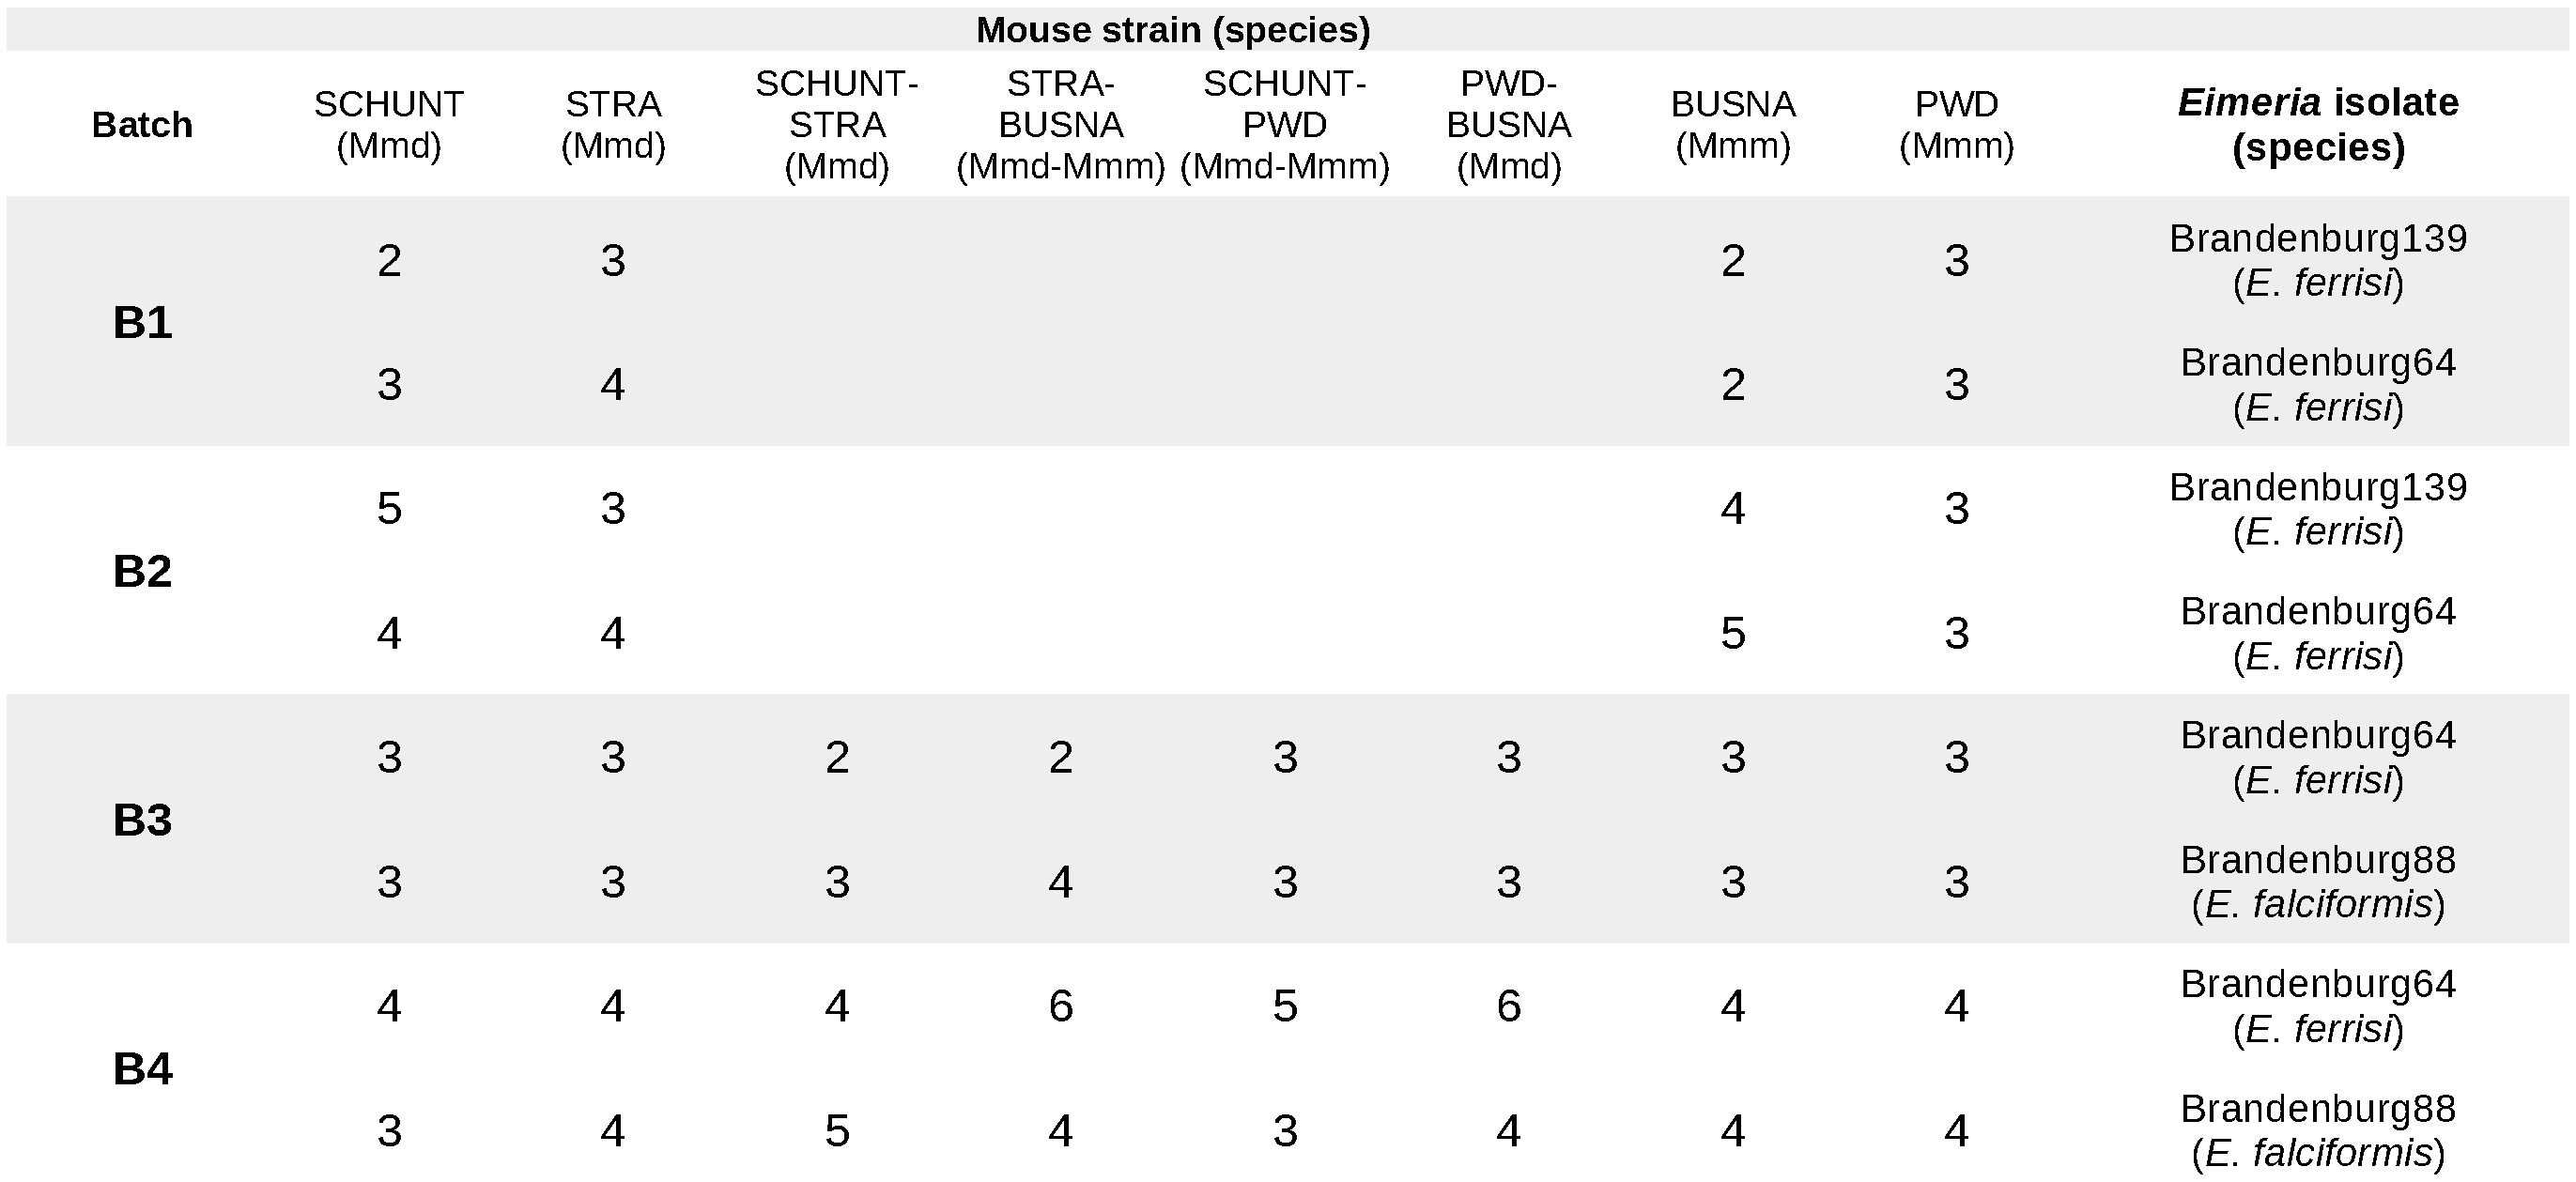
\includegraphics[width=\linewidth,height=\textheight,keepaspectratio]{images/3article2/SupplementaryTableS1.pdf}
	\captionsetup{labelformat=empty}
	\caption{\textbf{Supplementary Tabel S3.1.} Chronology of experimental infections.}
\end{figure}

\subsection*{Supplementary Material S3.2.} Conservative dataset.

\begin{figure}[H]
	\centering
	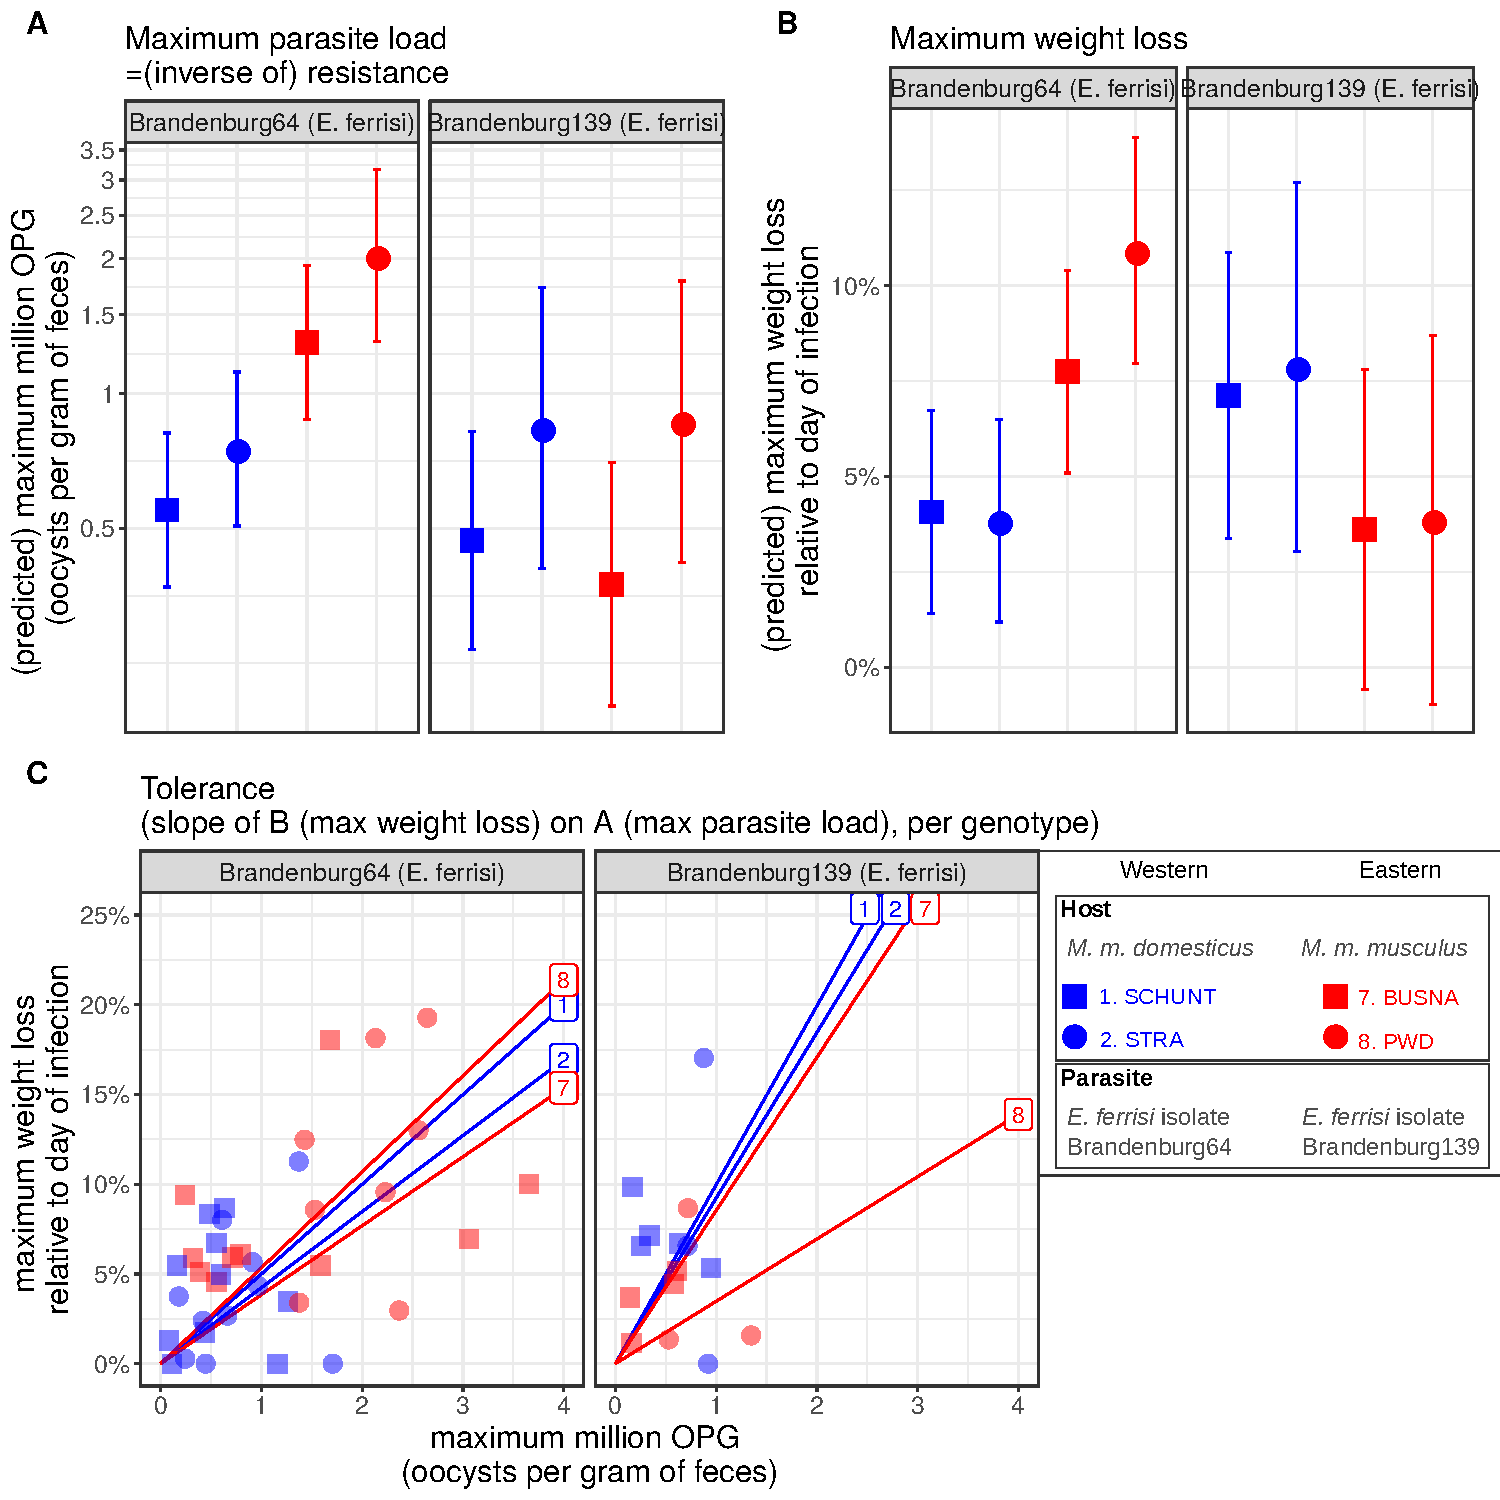
\includegraphics[width=\linewidth,height=\textheight,keepaspectratio]{images/3article2/SupplS2_Fig3.pdf}
	\captionsetup{labelformat=empty}
	\caption{\textbf{Supplementary Figure S3.2.1.} Comparison of resistance, impact on weight and tolerance between mouse strain for both \textit{Eimeria~ferrisi} isolates. (A) Maximum oocysts per gram of feces used as a proxy for (inverse of) resistance; (B) Impact on host health measured as the maximum weight loss during patent period relative to starting weight (\%); (C) Tolerance estimated by the slope of the linear regression with null intercept modelling maximum relative weight loss as a response of maximum oocysts per gram of feces. A steep slope corresponds to a low tolerance.
We did not detect (A) either higher parasite shedding of the Eastern parasite isolate in Eastern mouse strains and vice versa (LRT interaction factor mouse strain-parasite isolate: G=6.9, df=3, P=0.74) or (C) higher tolerance of Eastern hosts infected by Eastern parasite isolate and vice versa (LRT interaction factor mouse strain-parasite isolate: G=3.1, df=3, p=0.38), thus our results do not support the hypothesis of local adaptation between \textit{E.~ferrisi} and its host. }
\end{figure}

\begin{figure}[H]
	\centering
	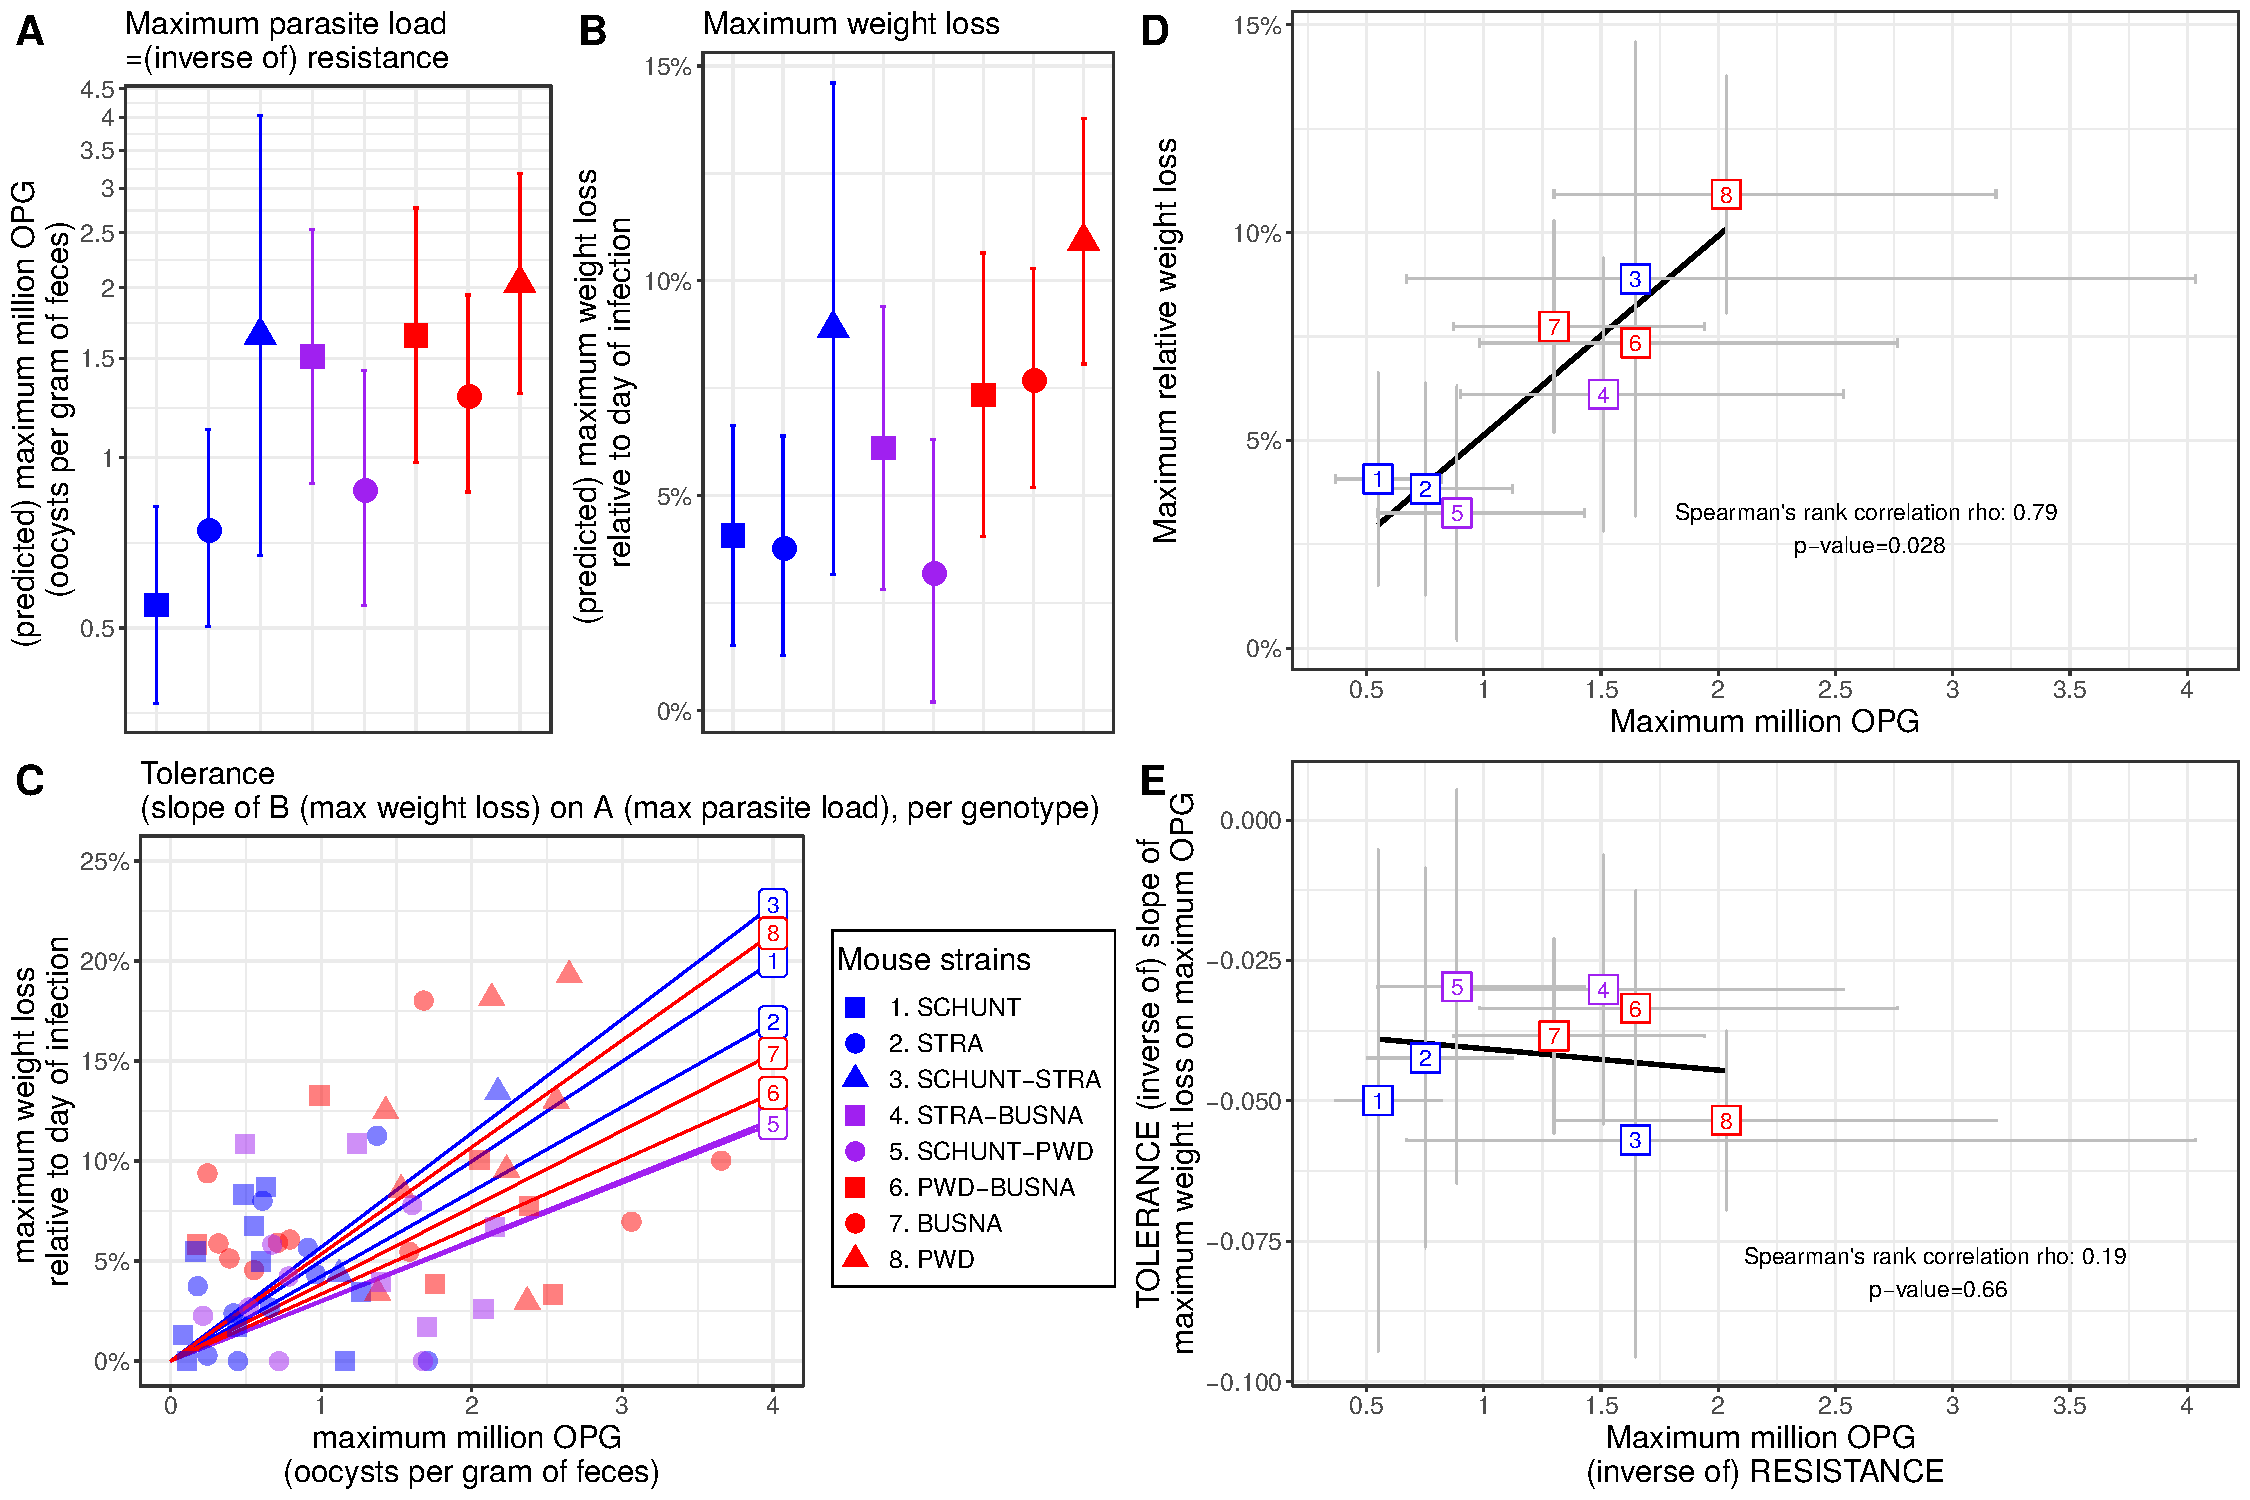
\includegraphics[width=\linewidth,height=\textheight,keepaspectratio]{images/3article2/SupplFig4.pdf}
	\captionsetup{labelformat=empty}
	\caption{\textbf{Supplementary Figure S3.2.1.} No indication of resistance-tolerance coupling for \textit{E.~ferrisi} isolate Brandenburg64. Colors represent mouse subspecies (blue: Mmd, red: Mmm, purple: Mmd-Mmm). Left side: comparison of maximum oocysts per gram of feces used as a proxy for (inverse of) resistance (A), impact on weight measured as the maximum weight loss during patent period relative to starting weight (B) and tolerance between mouse strains estimated by the slope of the linear regression with null intercept modelling maximum relative weight loss as a response of maximum oocysts per gram of feces, a steep slope corresponding to a low tolerance (C). Maximum number of OPG and relative weight loss differ between mouse strains (LRT: maximum number of OPG: G=22.6, df=7, p=0.002; maximum relative weight loss: G=21.7, df=7, p=0.0028), but tolerance is similar (LRT: G=5.4, df=7, p=0.62). Right side: non significant positive correlation between mean maximum oocysts per gram of feces and mean relative weight loss (D) and absence of correlation between maximum oocysts per gram of feces used as a proxy for (inverse of) resistance and tolerance (E); Grey error bars represent 95\% confidence intervals. Our results do not support coupling between resistance and tolerance \textit{E.~ferrisi} isolate Brandenburg64.}
\end{figure}

\begin{figure}[H]
	\centering
	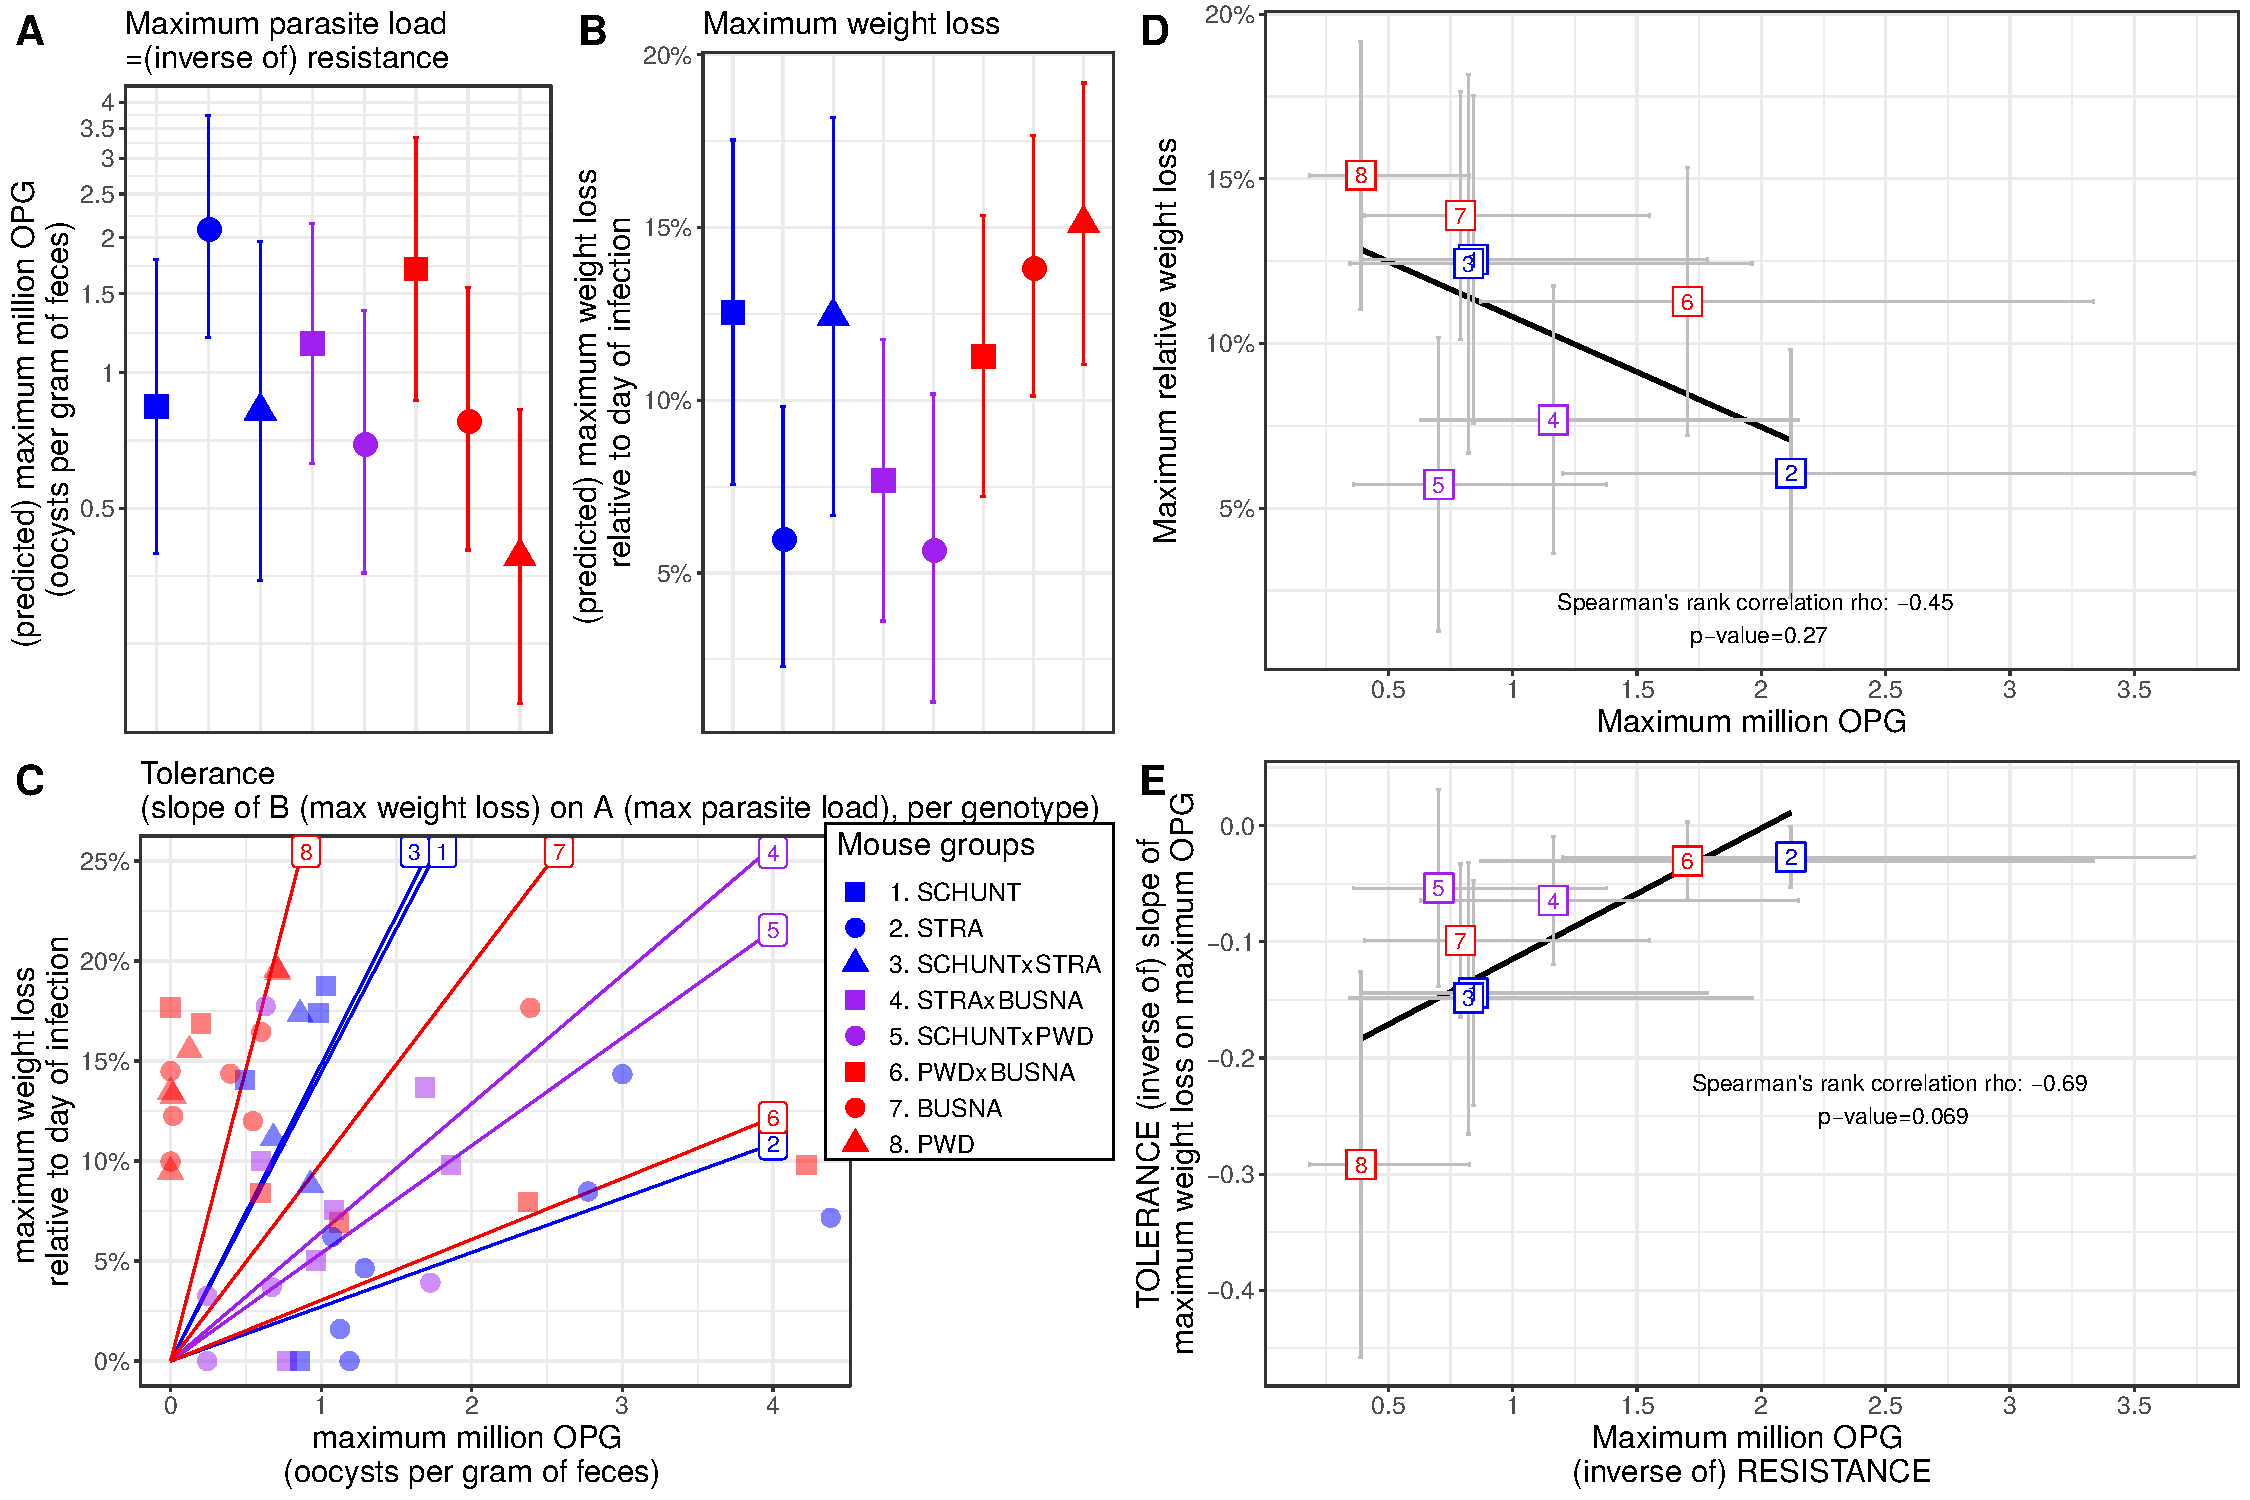
\includegraphics[width=\linewidth,height=\textheight,keepaspectratio]{images/3article2/SupplFig5.pdf}
	\captionsetup{labelformat=empty}
	\caption{\textbf{Supplementary Figure S3.2.1.} Coupling between resistance and tolerance for \textit{E.~falciformis} isolate Brandenburg88. Colors represent mouse subspecies (blue: Mmd, red: Mmm, purple: Mmd-Mmm). Left side: comparison of maximum oocysts per gram of feces used as a proxy for (inverse of) resistance (A), impact on weight measured as the maximum weight loss during patent period relative to starting weight (B) and tolerance between mouse strains estimated by the slope of the linear regression with null intercept modelling maximum relative weight loss as a response of maximum oocysts per gram of feces, a steep slope corresponding to a low tolerance (C). Maximum number of OPG, relative weight loss and tolerance differ between mouse strains (LRT: maximum number of OPG: G=24, df=14, p=0.046; maximum relative weight loss: G=20.1, df=7, p=0.005; tolerance: G=20.2, df=7, p=0.0051). Right side: non significant negative correlation between mean maximum oocysts per gram of feces and mean relative weight loss (D) and non significant negative correlation between maximum oocysts per gram of feces used as a proxy for (inverse of) resistance and tolerance (E); Grey error bars represent 95\% confidence intervals. Our results present indications of coupling between resistance and tolerance \textit{E.~falciformis} isolate Brandenburg88, with lower support than the full dataset likely due to the lower statistical power.}
\end{figure}


